\documentclass{beamer}
\mode<presentation>
\usetheme{boxes}

\usepackage{amsmath}
\usepackage{listings}
\usepackage{verbatim}

\lstset{%
showstringspaces=false,
numbers=left,
numbersep=10pt,
language=Ruby,
}
\title{The Count Distinct Problem}
\author{Steven Rosendahl}
\date{}
\begin{document}
\begin{frame}
\titlepage
\end{frame}

\section{The Problem}
\begin{frame}{The Question}
\begin{itemize}
\item What is the problem?
\pause
\item Image we have a set called $\mathbb{V}$ that contains a billion elements of the same type.
\pause
\item How many \textit{unique} elements are in $\mathbb{V}$?
\end{itemize}
\end{frame}

\begin{frame}{Questions}
\begin{enumerate}
\item \underline{Pok\'emon Problem:} How many unique Pok\'emon will a player encounter in a given playthrough of all the games?
\pause
\item \underline{Twitter Problem:} How many unique hashtags are made a day on Twitter?
\pause
\end{enumerate}
We will use $\mathbb{S}$ to represent the set of all the data, and $\mathbb{V}$ to represent the set of unique elements. 
\end{frame}

\section{The Hash Table}
\begin{frame}{Hashing}
\begin{itemize}
\item What is \textit{hashing}?
\pause
\item Applying a function $h(x)$ to every element in $\mathbb{S}$, and storing the result in $\mathbb{V}$.
\pause
\item Ideally, $h(x)$ is
\begin{enumerate}
\pause 
\item Onto (surjective)
\pause
\item One-to-one (injective)
\end{enumerate}
\pause
\item We can ignore the duplicate values in $\mathbb{V}$.
\end{itemize}
\end{frame}

\begin{frame}{Solving the Pok\'emon Problem}
\begin{itemize}
\item How can we solve the Pok\'emon Problem using a hash?
\pause
\item Create a hash function that turns a given Pok\'emon into a numerical value
\pause
\item Store the result in $\mathbb{V}$ if it is not already there.
\pause
\item The hash function:
\begin{enumerate}
\item Sum up the ASCII value of each character in a Pok\'emon's name. Call this $n$.
\pause
\item Add $n$ to the Pok\'emon's corresponding National Pok\'edex number. Call this $m$.
\pause
\item Find $m\ mod\ 721$.
\pause
\item Results:
\begin{itemize}
\pause
\item On average: 461 unique encounters
\end{itemize}
\end{enumerate}
\end{itemize}
\end{frame}

\begin{frame}[fragile]{Implementation}
\begin{lstlisting}[basicstyle=\small]
array.each do |pokemon|
     hash_table[pokemon.hash] = pokemon.hash
end
total = 0
hash_table.each do |val|
     if val != -1
          total = total + 1
     end
end
puts "The total number of unique encounters is #{total}"
\end{lstlisting}
\end{frame}

\begin{frame}{Problems With The Hash Table}
\begin{itemize}
\item Memory Intensive
\begin{itemize}
\item Pok\'emon problem only dealt with a set $\mathbb{S}$ of size 6000
\pause
\item Twitter Problem deals with $\mathbb{S}$ of size 200,000,000.
\pause
\item Collisions and collision policies also add to the amount of memory required.
\end{itemize}
\end{itemize}
\end{frame}

\section{The HyperLogLog}
\begin{frame}{The Algorithm}
\begin{enumerate}
\item Create a bitmap in memory. We will call this $\mathbb{V}$.
\pause
\item For each value $s$ is $\mathbb{S}$, hash $s$ to a binary number.
\pause
\begin{itemize}
\item We will use a \textit{Murmur Hash} to do this.
\end{itemize}
\pause
\item Analyze the first sequence of 0's in the binary value, and store the number of leading 0's into the bitmap.
\begin{itemize}
\item If the sequence of 0's has been seen before, there is a high probability that the term is a duplicate
\end{itemize}
\pause
\item Take the harmonic average of all the totals in the bitmap.
\end{enumerate}
\end{frame}

\begin{frame}{The Math}
\begin{itemize}
\item How much memory is required?
\pause
\[
\text{Memory Required} = \log_{2}{(\log_{2}{(M)})}
\]
\pause
\item $M$ is the size of the original set of data ($\mathbb{S}$).
\pause
\item For the Twitter Problem:
\pause
\begin{align*}
\text{Memory Required} &\approx \log_{2}{(\log_{2}{(200,000,000 \times 10)})}\\
&\approx 4.94 kb
\end{align*}
\pause
\item What is the predicted error?
\pause
\[
\text{Error} = \frac{\sqrt{3\log{(2)} - 1}}{m}
\]
\pause
\item $m$ is the number of spaces in the bitmap ($\mathbb{V}$).
\end{itemize}
\end{frame}

\begin{frame}{Solving the Twitter Problem}
\begin{itemize}
\item How can we process count 200,000,000 hashtags on an average computer?
\pause
\item We can lower the sample size and apply a best fit line to the data.
\begin{enumerate}
\pause
\item For 24 hours, gather 2000 tweets containing ``\#'' every 2 minutes.
\pause
\item Using the HyperLogLog, determine the unique number of total hashtags every time a new sample is gathered.
\end{enumerate}
\end{itemize}
\end{frame}

\begin{frame}[fragile]{Implementation}
\begin{lstlisting}[language=Ruby]
mhll = Hyperll::HyperLogLog.new(10)
File.open("twitter_data.txt","r") do |file|
     file.each_line do |line|
          mhll.offer line
     end
end
str = "Unique Elements: #{mhll.cardinality}"
puts str
\end{lstlisting}
\end{frame}

\begin{frame}{Results}
\begin{figure}
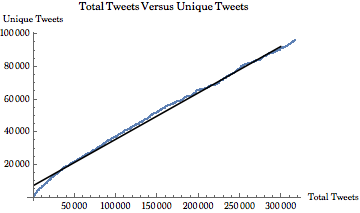
\includegraphics[scale=0.7]{twitter_problem/resultspng}
\caption{$0.284356 x + 7361.39$}
\end{figure}
\pause
\begin{itemize}
\item Plugging in 200,000,000 gives us
\pause
\item $5.68785\times10^7$ unique hashtags.
\end{itemize}
\end{frame}
\end{document}